\documentclass[./main.tex]{subfiles}

\begin{document}
\onehalfspacing
\section{Բազմությունների դեկարտյան (ուղիղ) արտադրյալ, արտա\-պատ\-կերում\-ների ուղիղ արտադրյալ, անկյունագծային արտապատկերում։ Համարժեքութ\-յան հարա\-բերու\-թյուն բազմության վրա, ֆակտոր-բազմություն։}\label{sec:2}

Գոյություն ունի տրված բազմության կամ մի քանի բազմությունների միջոցով նոր բազ\-մու\-թյուն կառուցելու
երեք հիմնական եղանակ։ Դրանք են՝
\begin{enumerate}
    \item [ա)] բազմությունից ենթաբազմության առանձնացումը,
    \item [բ)] բազմությունների ուղիղ (դեկարտյան) բազմապատկումը,
    \item [գ)] տվյալ բազմության ֆակտոր-բազմության կառուցումը։
\end{enumerate}
\par Սրանցից առաջինը քննարկվեց \hyperref[sec:1]{թեմա 1}-ում։ Այժմ մյուս երկուսը։ 
% ավելացված
\par Երկու՝ $A$ և $B$ ոչ դատարկ \textbf{բազմությունների դեկարտյան} կամ \textbf{ուղիղ արտա\-դր\-յալ} կոչվում է այն բազմությունը (նշանակվում է $A \times B$), որի տարրերը բոլոր $(a,b)$ կարգավորված զույգերն են, որտեղ $a\in A$, $b \in B$: 
\par Մի քանի $A_1,\dots,A_n$ ոչ դատարկ \textbf{բազմությունների ուղիղ արտադրյալ} կոչվում է $\left\{(a_1,\dots, a_n)\mid a_1\in A_1,\dots, a_n \in A_n\right\}$ բազմությունը և նշանակվում է $A_1\times \dots \times A_n$ կամ $\prod\limits_{i=1}^n A_i$։ Այստեղ $(a_1, \dots, a_n)$-ը $A_1,\dots, A_n$ բազմություններից մեկական վերցրած տարրերի հաջորդականություն է։ Մասնավոր դեպքում, երբ $A_1=\dots=A_n=A$, նրանց ուղիղ արտադրյալը նշանակվում է $A^n$։ Եթե $A_1,\dots, A_n$ բազմություններից որևէ մեկը դատարկ բազմություն է, ապա նրանց արտադրյալ է համարվում $\varnothing$ դատարկ բազմությունը։ 
\begin{theorem}
 Կամայական $A$, $B$, $C$, $D$-ն ոչ դատարկ բազմութ\-յուն\-ների համար տեղի ունեն հետևյալ համարժեքությունները․
\begin{enumerate}
    \item [ա)] $(A\times C=B\times D)\Leftrightarrow A=B$ և $C=D$
    \item [բ)] $(A\times C\subset B\times D)\Leftrightarrow A\subset B$ և $C\subset D$։
\end{enumerate}
\end{theorem}
\label{թեորեմ 2:1}
% ավելացված
\par Երկու պնդումներն էլ անմիջականորեն հետևում են սահմանումներից։
\begin{example}
Դիտարկենք $\underbrace{\mathbb{R}\times\dots \times \mathbb{R}}_n$ արտադրյալը (որտեղ $\mathbb{R}$-ը թվային ուղիղն է) կազմված իրական թվերի բոլոր $(r_1,\dots,r_n)$ հաջորդականություններից։ Այն կա\-րող է նույնացվել $n$-չա\-փա\-կա\-նու\-թյան $\mathbb{R}^n$ կոորդինատային գծային տարածության բոլոր կետերի բազմու\-թյան հետ։%1
\end{example}
\label{օրինակ 2:1}
\par Որպեսզի պարզ լինի հաջորդ օրինակը, դիտարկենք այն մակերևույթը, որն առա\-ջա\-նում է, երբ որևէ շրջանագիծ, օրինակ՝ $(2,0)$ կենտրոնով և $1$ շառավղով $(x-2)^2+y^2=1$ շրջանագիծը, պտտվում է նրան չհատող $OY$ առանցքի շուրջը $\R^3$ տարածության մեջ՝ կատարելով մեկ լրիվ պտույտ։ Այսպիսի մակերևույթները կոչվում են \textbf{տոր} և ունեն փրկարար օղակի տեսք։ 
% ավելացված
Պարզ է, որ շրջանագծի ամեն մի $(x,y)$ կետ պտույտի ընթացքում գծում է շրջանագիծ։ Այն կոչվում է \textbf{տորի զու\-գա\-հե\-ռական}։ Տորն ամբողջովին ծածկված է իր զուգահեռականներով։ Պարզ է նաև, որ $OY$ առանցքով անցնող ամեն մի հարթություն հատում է տորը շրջանագծով։ Դրանք նույնպես ամբողջովին ծածկում են տորը և կոչվում են \textbf{տորի միջօրեականներ}։
\par Նկատենք, որ տորի որևէ սևեռված $A$ կետից կարելի է տեղափոխվել տորի ցանկացած այլ կետ՝ կատարելով տարածության մեջ երկու պտույտ $\alpha, \beta \in [0, 2\pi)$ անկյուններով։ Ստորև նկարում $\alpha$ և $\beta$ անկյուն\-ները պատկերված են տորի զու\-գա\-հե\-ռականների և միջօրեականների $AB$ և $BC$ աղեղների տեսքով։ Ընդ որում, աղեղները հաշվարկվում են սևեռված $A$ կետից, սևեռ\-ված ուղղություններով և սևեռ\-ված հաջորդականությամբ: Այժմ տորի $C$ կետ տեղափոխվելու համար նախ $A$ կետից ան\-ջատ\-վում է $\alpha$ աղեղ զուգահեռականով, այնուհետև $B$ կետից՝ $\beta$ աղեղ միջօրեականով։ Այսպի\-սով կամայական տորի ցանկացած կետ միարժեքորեն ինդեք\-սա\-վորվում է $(\alpha, \beta)$ թվազույգով, որտեղ $\alpha, \beta \in [0, 2\pi)$։

\begin{tikzpicture}
\node (russell) at (0,0)
    {
\begin{tikzpicture}[anchor=center]
% x - coords
%\node[anchor=north] at (0.5, 0) {$(1;0)$};
\node[anchor=north] at (-0.5, 0) {$0$};
\node[anchor=north] at (2, 0) {$(2,0)$};

% circle
\draw[very thick] (2,0) circle (1cm);

%points on y axes
\filldraw (1,0) circle (2.5pt);
\filldraw (2,0) circle (2.5pt);
\filldraw (3,0) circle (2.5pt);

% axis names
\node[anchor=west] at (4, 0) {$X$};
\node[anchor=south] at (0, 2) {$Y$};

\draw[->, semithick] (-1,0) -- (4, 0);
\draw[->, semithick] (0,-1) -- (0, 2);
\end{tikzpicture}
};
\node (whitehead) at (8,0)
    {\includegraphics[scale=0.1]{images/id4.png}};
\node[anchor=north] at (6.85, -0.25) {$A$};
\node[anchor=north] at (9.1, 0.4) {$B$};
\node[anchor=north] at (9.82, -0.57) {$C$};
\draw[->, thick] (8.1, -0.527) -- (8.12, -0.527);
\draw[->, thick] (9.46, -0.38) -- (9.51, -0.44);
\draw[->, thick] (russell.east) -- (whitehead.west);
\end{tikzpicture}

\begin{example}
Դիտարկենք $S\times S$ ուղիղ արտադրյալը, որտեղ $S$-ը
% $O(0,0)$ կենտրոնով և $1$ շառավղով $\{(x_1,x_2) \in \R^2 \mid x_1^2+x_2^2=1\}$ շրջանագիծն է։ 
% ավելացված
որևէ սևեռված շրջանագծի բոլոր կետերի բազմությունն է։ Այն կոչվում է \textbf{վերացական տոր}։ Ցույց տանք, որ գոյություն ունի փոխմիարժեք համապատասխանություն $S\times S$ վերա\-ցա\-կան տորի բոլոր կետերի և կամայական տորի (որպես մակերևույթի) բոլոր կետերի միջև։%3
\par \hyperref[sec:1]{Թեմա 1}-ի \hyperref[օրինակ 1:4]{օրինակ 4}-ից գիտենք, որ կամայական $S$ շրջանագծի կետերը կարելի է ինդեքսավորել բոլոր $[0,2\pi)$ անկյուններով։ Հետևաբար $S\times S$-ի կետերը կարելի է ինդեքսավորել բոլոր $(\alpha, \beta )$ թվա\-զույ\-գե\-րով, որտեղ $\alpha ,\beta \in [0,2\pi)$։ Բայց ինչպես տեսանք, կամայական տորի կետերը նույնպես ինդեքսավորվում են այդպիսի թվա\-զույ\-գերով։ Ուստի ցանկացած տոր կարող է դիտվել որպես $S\times S$ վերացական տորի \textbf{երկրաչափական մոդել}։
% \par Ասվածը պարզաբանենք տեսողաբար։ Վերը նշված գծագրում $\alpha$ և $\beta$ անկյուն\-ները պատկերված են տորի զուգահեռականների և միջօրեականների (դրանք շրջա\-նագծեր են) աղեղների տեսքով։ Ընդ որում աղեղները հաշվարկվում են սևեռված $A$ կետից, սևեռված ուղղություններով և սևեռված հաջորդականությամբ․ նախ ան\-ջատ\-վում է $\alpha$ աղեղ զուգահեռականով, այնուհետև՝ $\beta$ աղեղ միջօրեականով։ Այսպի\-սով տորի վրա ունենք կորագիծ կոորդինատային համակարգ $A$ սկզբնակետով։
\end{example}
\label{թեորեմ 2:2}

\begin{example}
\textbf{Կրկնակի ճոճանակ} կոչվում է միմյանց հետ շարժական ձևով միաց\-ված $a$ և $b$ ձողերից կազմված սարքը։ Դրանցից $a$-ն ազատ պտտվում է իր $O$ անշարժ ծայրակետի շուրջը, իսկ $b$-ն՝ $a$-ի հետ միացման շարժական կետի շուրջը։ Հեշտ է տեսնել, որ գոյություն ունի փոխմիարժեք համապատասխանություն կրկնակի ճոճանակի բոլոր $M(\alpha,\beta)$ դիրքերի բազմության և տորի բոլոր կետերի բազմության միջև։
\begin{center}
\begin{tikzpicture}
\draw[-, semithick] (-1,0) -- (6, 0);
\draw[-, semithick] (0,-1) -- (0,5);

\filldraw (5,3) circle (2.5pt);

\draw[-, semithick] (5,1) -- (5, 5);
\draw[-, semithick] (3,3) -- (7, 3);

\node[anchor=north west] at (3.65,4.85) {$M$};
\node[anchor=north east] at (0,0) {$O$};

 \draw
  (1,0) coordinate (a)
  -- (0,0) coordinate (b)
  -- (5,3) coordinate (c)
   pic["$\alpha$",draw=orange,->,very thick, angle eccentricity=1.2,angle radius=1.5cm] {angle=a--b--c};
   
\draw[semithick] (0,0) coordinate (o) -- (5,3) coordinate (m);
\node[anchor=south] at (2.5,1.5) {$a$};

\coordinate (center) at (5,3);
  \def\radius{1.5cm}
  % a circle
  \draw (center) circle[radius=\radius];

  % a random point of the circl
\draw
  (7,3) coordinate (a)
  -- (5,3) coordinate (b)
  -- ++(2/3*180:\radius) coordinate (c)
  pic["$\beta$",draw=orange,->,very thick, angle eccentricity=1.2,angle radius=0.65cm] {angle=a--b--c};
  
\node at (4.5,3.5) {$b$};

\end{tikzpicture}
\end{center}
\end{example}
\label{օրինակ 2:3}
\par Դիցուք $X$-ը կամայական բազմություն է, իսկ $I$-ն $[0,1]$ հատվածն է։ $X\times I$ ուղիղ արտադրյալը կոչվում է \textbf{գլան $\boldsymbol{X}$ հիմքով}։ Նրա $X\times \{0\}$ և $X\times \{1\}$ ենթա\-բազմութ\-յուն\-ները կոչվում են \textbf{գլանի ստորին} և \textbf{վերին հիմքեր}։ Մասնավոր դեպքում, երբ $X$-ը որևէ հարթ պատկեր է, $X\times I$ բազմությունը երկ\-րա\-չա\-փո\-րեն կարող է պատկերվել որպես գլանաձև մարմին $\mathbb{R}^3$-ում։ 
\begin{example}
Ստորև պատկերված է $X \times I$ տեսքի մարմին $\R^3$-ում: Նրա $X$ հիմքն ունի հարթության շրջանաձև տիրույ\-թի տեսք, որից հեռացված են երկու ավելի փոքր շրջանաձև տիրույթներ։
\begin{center}
\includegraphics[scale=0.15]{images/id 6.png}
\end{center}
\end{example}%5
\label{օրինակ 2:4}
\begin{theorem}
Ցանկացած $A,B,C,D$ բազմությունների դեպքում
\begin{enumerate}
    \item [ա)] $(A\times B)\cap (C\times D)=(A\cap C)\times (B\cap D)$,
    \item [բ)] $(A\times B)\cup (C\times D)\subset (A\cup C)\times (B\cup D)$,
    \item [գ)] $(A\cup B)\times C=(A\times C)\cup (B\times C)$,
    \item [դ)] $(A\setminus B)\times C=(A\times C)\setminus (B\times C)$։
\end{enumerate}
\end{theorem}
\label{թեորեմ 2:2}
\begin{proof}
Ապացուցենք բ)-ն՝ մյուսները թողնելով ընթերցողին․
\begin{equation*}
\begin{aligned}
x&\in (A\times B)\cup (C\times D)\ \Leftrightarrow \
\begin{sqcases} x\in A\times B \\ x\in C\times D \end{sqcases}\hspace{-1em}
\ \Leftrightarrow \
\begin{sqcases}
\exists a\in A \textrm{ և } b\in B, \textrm{ որ } x=(a,b)\\
\exists c\in C \textrm{ և } d\in D, \textrm{ որ } x=(c,d)
\end{sqcases}\hspace{-1em} \Rightarrow \\
& \Rightarrow\ \begin{sqcases}
a\in A\cup C \textrm{ և } b\in B \cup D \\
c\in A\cup C \textrm{ և } d\in B\cup D
\end{sqcases}\hspace{-1em}
\ \Leftrightarrow\
\begin{sqcases}
(a,b)\in (A\cup C)\times(B\cup D)\\
(c,d)\in (A\cup C)\times(B\cup D)
\end{sqcases}\hspace{-1em} \ \Leftrightarrow\\
& \Leftrightarrow\ x\in (A\cup C)\times(B\cup D)\ \Leftrightarrow\ \left((A\times B)\cup (C\times D)\right)\subset \left((A\cup C)\times (B\cup D)\right)
\end{aligned}
\end{equation*}
\end{proof}
\par Նկատենք, որ ընդհանուր դեպքում $(A\times B)\cup (C\times D)\neq (A\cup C)\times(B\cup D)$։ Դա ցույց տալու համար բերենք օրինակ։

\begin{center}
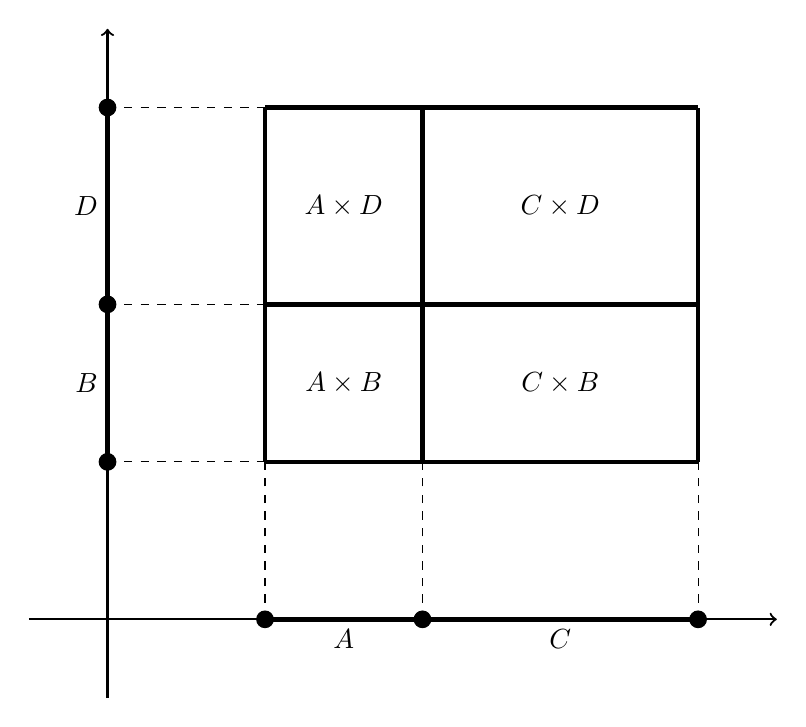
\begin{tikzpicture}
\node[anchor=east] at (0, 3) {$B$};
\node[anchor=east] at (0, 5.25) {$D$};
\node[anchor=north] at (3, 0) {$A$};
\node[anchor=north] at (5.75,0) {$C$};
\node at (3, 3) {$A\times B$};
\node at (5.75, 5.25) {$C\times D$};
\node at (5.75, 3) {$C\times B$};
\node at (3, 5.25) {$A\times D$};
%points on y axes
\filldraw (2,0) circle (3pt);
\filldraw (4,0) circle (3pt);
\filldraw (7.5,0) circle (3pt);
%points on y axes
\filldraw (0,2) circle (3pt);
\filldraw (0,4) circle (3pt);
\filldraw (0,6.5) circle (3pt);

\draw[->, thick] (-1,0) -- (8.5, 0);
\draw[ultra thick] (2,0) -- (7.5, 0);
%dashed lines on x axes
\draw[dashed] (2,0) -- (2, 2) node[anchor=north east] at (2,2) {};
\draw[dashed] (4,0) -- (4, 2);
\draw[dashed] (7.5,0) -- (7.5, 2);
%thick lines on x axes
\draw[ultra thick] (2,2) -- (2, 6.5);
\draw[ultra thick] (4,2) -- (4, 6.5);
\draw[ultra thick] (7.5,2) -- (7.5, 6.5) node[anchor=north west] at (7.5,2) {};

\draw[->, thick] (0,-1) -- (0, 7.5);
\draw[ultra thick] (0,2) -- (0, 6.5);
\draw[dashed] (0,2) -- (2, 2);
\draw[dashed] (0,4) -- (2, 4);
\draw[dashed] (0,6.5) -- (2, 6.5) node[anchor=south east] {};
%thick lines on y axes
\draw[ultra thick] (2,2) -- (7.5, 2);
\draw[ultra thick] (2,4) -- (7.5, 4);
\draw[ultra thick] (2,6.5) -- (7.5, 6.5) node[anchor=south west] {};
\end{tikzpicture}
\end{center}

\par Գծագրում $A,B,C,D$-ն թվային ուղղի հատվածներ են, բ)-ի ձախ մասը $A\times B$ և $C\times D$ ուղղանկյունների միա\-վո\-րումն է, աջ մասը՝ $A\times B$, $A \times D$, $C \times B$, $C \times D$ ուղղանկյունների միավորումն է, և դրանք նույնը չեն։ \qed
\par Բազմությունների $X\times Y$ արտադրյալի համար սահմանվում են $P_X:X \times Y \rightarrow X$ և $P_Y:X\times Y\rightarrow Y$ արտապատկերումներ $P_X(x,y)=x$ և ${P_Y(x,y)=y}$, $(x,y) \in X\times Y$ բանաձևերով։ Դրանք կոչվում են  $X \times Y$-ի \textbf{կանոնական պրոյեկցիա\-ներ} համապատասխանաբար առաջին և երկրորդ արտադրիչների վրա։
\par Այժմ քննարկենք երկու $\textbf{արտապատկերումների արտադրյալ}$ հասկացությունը․ եթե ունենք $f_1:X_1 \rightarrow Y_1$ և $f_2:X_2 \rightarrow Y_2$ արտապատկերումներ, ապա սահմանվում է $f_1\times f_2:X_1\times X_2\rightarrow Y_1\times Y_2$ արտապատկերում՝ $(f_1\times f_2)(x_1,x_2)=(f_1(x_1),f_2(x_2))$ բանաձևով (կոչվում է $f_1$-ի և $f_2$-ի արտադրյալ)։ Այս $f_1$, $f_2$, $f_1 \times f_2$ արտա\-պատ\-կե\-րում\-ները և կանոնական պրոյեկցիաները միմյանց հետ կապվում են երկու կոմուտատիվ դիագրամով՝
\begin{center}
\begin{tikzcd}[row sep=large, column sep = huge]
X_1\times X_2 \arrow{r}{f_1\times f_2} \arrow{d}[swap]{P_{X_1}}    
& Y_1\times Y_2 \arrow{d}{P_{Y_1}} \\
X_1 \arrow{r}{f_1}
& Y_1
\end{tikzcd}\qquad
\begin{tikzcd}[row sep=large, column sep = huge]
X_1\times X_2 \arrow{r}{f_1\times f_2} \arrow{d}[swap]{P_{X_2}}    
& Y_1\times Y_2 \arrow{d}{P_{Y_2}} \\
X_2 \arrow{r}{f_2}
& Y_2
\end{tikzcd}
\end{center}
\par Առաջին դիագրամի կոմուտատիվությունը նշանակում է, որ $P_{Y_1}\circ(f_1\times f_2)$ և ${f_1\circ P_{X_1}}$ համադրույթները որոշում են միևնույն $X_1\times X_2\rightarrow Y_1$ արտապատկե-\linebreak րումը, իսկ երկրորդ դիագրամի կոմուտատիվությունը նշանակում է, որ նույնն են $P_{Y_2}\circ {(f_1 \times f_2)}$ և $f_2\circ P_{X_2}$ համադրույթները։
\par Ցույց տանք առաջինի կոմուտատիվությունը․ կա\-մա\-յա\-կան $(x_1,x_2)\in X_1\times X_2$ տարրի համար մի կողմից ունենք
\[(P_{Y_1}\circ (f_1 \times f_2))(x_1,x_2)=P_{Y_1}\circ ((f_1 \times f_2)(x_1,x_2))=P_{Y_1}(f_1(x_1),f_2(x_2))=f_1(x_1),\] իսկ մյուս կողմից ունենք
\[(f_1 \circ P_{X_1})(x_1,x_2)=f_1(P_{X_1}(x_1,x_2))=f_1(x_1)։\]
Ուստի $P_{Y_1} \circ (f_1\times f_2)=f_1 \circ P_{X_1}$։ \qed
\par Այնուհետև, $f_1 \times f_2$-ի նմանությամբ սահմանվում է բազմությունների ցանկացած վերջավոր (անգամ անվերջ) քանակով $f_i:X_i\rightarrow Y_i$ արտապատկերումների
\[f_1\times f_2 \times \dots  \times f_n:X_1 \times X_2 \times \dots  \times X_n\rightarrow Y_1\times Y_2\times \dots  \times Y_n\]
արտադրյալը՝
\[(f_1 \times f_2 \times \dots  \times f_n)(x_1, x_2, \dots, x_n)=(f_1(x_1), f_2(x_2), \dots, f_n(x_n)), \quad \text{որտեղ } x_i \in X_i\]
բանաձևով։
\begin{theorem}
Դիցուք ունենք $f_1:X_1\rightarrow Y_1,\ f_2:X_2 \rightarrow Y_2$ կամայական ար\-տա\-պատ\-կե\-րում\-ներ։ Ապա
\begin{enumerate}
    \item [ա)] ցանկացած $A_1 \subset X_1,\ A_2 \subset X_2$ ենթաբազմությունների դեպքում \\ $(f_1 \times f_2)(A_1 \times A_2)=f_1(A_1)\times f_2(A_2)$,
    \item [բ)] ցանկացած $B_1 \subset Y_1$ և $B_2 \subset Y_2 $ ենթաբազմությունների դեպքում\\ $(f_1 \times f_2)^{-1}(B_1\times B_2)=f_1^{-1}(B_1)\times f_2^{-1}(B_2)$։
\end{enumerate}
\end{theorem}
\label{թեորեմ 2:3}
\begin{proof}
Ապացուցենք բ)-ն՝ թողնելով ա)-ի ապացուցումը ընթերցողին․\\
$(x_1,x_2)\in (f_1\times f_2)^{-1}(B_1\times B_2)\ \Rightarrow \ (f_1 \times f_2)(x_1,x_2)\in B_1 \times B_2\ \Rightarrow\ (f_1(x_1),f_2(x_2)) \in B_1\times B_2\ \Rightarrow\ f_1(x_1) \in B_2 $ և $f_2(x_2)\in B_2\ \Rightarrow\ x_1 \in f_1^{-1}(B_1)$ և $x_2 \in f_2^{-1}(B_2)\ \Rightarrow\ (x_1,x_2)\in f_1^{-1}(B_1)\times f_2^{-1}(B_2)$։
Այսպիսով ստացանք, որ $(f_1\times f_2)^{-1}(B_1\times B_2) \subset f_1^{-1}(B_1)\times f_2^{-1}(B_2) $։ Հակառակ ներդրումը հետևում է նրանից, որ իրականում բոլոր $\Rightarrow$ անցումները հա\-մար\-ժե\-քու\-թյուն\-ներ են։
\end{proof} 
\par Այժմ դիտարկենք արտապատկերումների ևս մի կառույց։ Եթե ունենք\linebreak $f_1:X \rightarrow Y_1$ և $f_2:X\rightarrow Y_2 $ արտապատկերումներ, որոնց որոշման տիրույթները նույն $X$ բազմությունն է, ապա սահմանվում է $X \rightarrow Y_1 \times Y_2$ արտապատկերում $x \mapsto (f_1(x),f_2(x))$ համադրումով։
\par Այդ արտապատկերումը նշանակվում է $(f_1,f_2):X\rightarrow Y_1 \times Y_2$ և կոչվում է $f_1\textrm{-ով}$ և $f_2$-ով ծնված $\textbf{անկյունագծային արտապատկերում}$։ Այս\-պի\-սով $(f_1,f_2)(x)=(f_1(x),f_2(x))$։ 
\par Անկյունագծային արտապատկերում անվանումը պայմանավորված է նրանով, որ մասնավոր $X=Y_1=Y_2=[a,b]$, $f_1=f_2=\nuynakan_{[a,b]}$ դեպքում $[a,b]$ հատվածի կերպարը $(f_1,f_2)$ արտապատկերման դեպքում $[a,b]\times [a,b]$ քառակուսու\linebreak $\{(x,x)\mid x\in [a,b]\}$ անկյունագիծն է։
% Անկյունագծային արտապատկերում անվանումը պայմանավորված է նրանով, որ մասնավոր $X=Y_1=Y_2=[a,b]$, $f_1=f_2=\nuynakan_{[a,b]}$ դեպքում $[a,b]$ հատվածի $(f_1,f_2)([a,b])$ կերպարը $[a,b]\times [a,b]$ քառակուսու $\{(x,x)\mid x\in [a,b]\}$ անկյունագիծն է։
\par Նման ձևով սահմանվում է ցանկացած վերջավոր (անգամ անվերջ) քանակով $f_i:X\rightarrow Y_i,\ i=1,2,\dots ,n$ ար\-տա\-պատ\-կեր\-ում\-նե\-րով ծնված անկյունագծային $(f_1,f_2,\dots ,f_n):X\rightarrow Y_1 \times Y_2 \times \dots \times Y_n$ արտապատկերումը՝ $(f_1,f_2,\dots ,f_n)(x)=(f_1(x),f_2(x),\dots ,f_n(x))$ բանաձևով։
\begin{theorem} 
Ունենք $f_1:X\rightarrow Y_1$ և $f_2:X\rightarrow Y_2$ արտապատկերումներ։ Ապա
\begin{enumerate}
    \item[ա)] ցանկացած $A\subset X$ ենթաբազմության դեպքում $(f_1,f_2)(A)\subset f_1(A)\times f_2(A)$,
    \item[բ)] ցանկացած $B_1\in Y_1$ և $B_2 \in Y_2$ ենթաբազմությունների դեպքում \\
$(f_1,f_2)^{-1}(B_1\times B_2)=f_1^{-1}(B_1)\cap f_2^{-1}(B_2)$։
\end{enumerate}
\end{theorem}
\label{թեորեմ 2:4}
\begin{proof}
Ապացուցենք բ)-ն։
\begin{align*}
& x\in (f_1,f_2)^{-1}(B_1\times B_2)\ \Leftrightarrow \ (f_1,f_2)(x) \in B_1\times B_2 \ \Leftrightarrow \ (f_1(x_1),f_2(x_2)) \in B_1\times B_2 \\
& \Leftrightarrow \ f_1(x)\in B_1 \textrm{ և } f_2(x)\in B_2\ \Leftrightarrow \ x \in f_1^{-1}(B_1) \textrm{ և } x \in f_2^{-1}(B_2) \ \Leftrightarrow\ x \in f_1^{-1}(B_1) \cap f_2^{-1}(B_2)։
\end{align*}
\end{proof}
\par Այժմ սահմանենք բազմության ֆակտոր-բազ\-մու\-թյուն հասկացությունը։
% \par Քանի որ մեզ համար սրանցից հիմնականն ու առաջնայինը ֆակտոր-բազմու\-թյան հասկացությունն է, սկսենք դրանից։
\par Դիցուք՝ $X$ բազմությունը ներկայացված է իր մի քանի զույգ առ զույգ չհատվող, ոչ դատարկ $X_i$ ենթաբազմությունների միավորման տեսքով՝ $X=\cup X_i$։ Այսպիսով ${X_i \subset X},\ X_i\neq \varnothing$ ցանկացած $i\in I$ ինդեքսի դեպքում և $X_i\cap X_j=\varnothing$ ցանկացած $i\neq j$ դեպքում։
\par Այս դեպքում ասում են, որ ունենք $X$ \textbf{բազմության տրոհում} $\{X_i\},\ i\in I$ ենթա\-բազ\-մու\-թյունների։
\par Դիտարկենք նոր՝ $F(X)$ բազմություն (բազմությունների ընտանիք), որի տար\-րե\-րը $X$-ի $X_i$ ենթաբազմու\-թյուն\-ներն են։ Այն կոչվում է $X$ բազմության \textbf{ֆակտոր-բազմու\-թյուն՝ ծնված $X$-ի տվյալ տրոհումով}։
% ըստ $\{X_i\} $ տրոհման։

\begin{example}
Դիցուք $X$-ը ԵՊՀ բոլոր ուսանողների բազմությունն է, իսկ $X_1$, $X_2$, $\dots$, $X_{20}$-ը նրա ենթաբազմություններն են ըստ ֆակուլտետների (համարենք, որ տվյալ պահին ֆակուլտետների քանակը $20$ է)։ Այս դեպքում $F(X)=\{X_1,X_2,\dots,X_{20}\}$։
\par Պատկերավորության համար թույլ տալով մեզ որոշ ազատություն՝ կարող ենք $F(X)$-ը նույնացնել ԵՊՀ-ի բոլոր ֆակուլտետների բազմության հետ։
\par Նկատենք, որ նույն $X$ բազմությունից կարելի է ստանալ նաև այլ ֆակտոր-բազ\-մու\-թյուն\-ներ։
Դիտարկելով ԵՊՀ ուսանողների բազմության տրոհումը ըստ կուրսերի ($1$-ին, $2$-րդ, $3$-րդ, $4$-րդ կուրսեր բա\-կա\-լավ\-րիա\-տում և $5$-րդ, $6$-րդ կուրսեր մա\-գիստ\-րա\-տու\-րա\-յում)՝ կստանանք մի նոր ֆակտոր-բազմություն, որի տարրերը կարելի է ինդեքսավորել բնական թվերի բազմության $\{1,2,3,4,5,6\}$ ենթաբազմության տար\-րե\-րով։
\par Քննարկված երկու դեպքերից յուրաքանչյուրում, ելնելով պատկերավորության նկատառումներից՝ ֆակտոր-բազմությունը ներկայացրինք \textbf{մոդելի} միջոցով։ Մոդելի ընտրությունը նպատակահարմարության կամ ճաշակի հարց է։ Բայց պարտադիր է, որ հաստատված լինի որոշակի փոխմիարժեք համապատասխանություն իրական ֆակտոր-բազմության և տվյալ մոդելի տարրերի միջև։
\end{example}
\label{օրինակ 2:5}
\par Դիցուք ունենք $X$ բազմություն, նրա որևէ $\{X_i,\, i\in I\}$ տրոհում, և $F(X)$-ը $X$-ի ֆակտոր-բազմությունն է։ Սահ\-ման\-վում է $P:X \rightarrow F(X)$ \textbf{կանոնական արտա\-պատ\-կե\-րում}․ որպես $x\in X$ կետի $P(x)$ կերպար վերցվում է $F(X)$-ի այն $X_i$ տարրը, որ $x\in X_i$։ Պարզ է, որ $P$-ն սյուրյեկտիվ արտապատկերում է, և $F(X)$-ի տարրերի նա\-խա\-կեր\-պար\-նե\-րը որոշում են $X$-ի $\{X_i\}$ տրոհումը։ Այսպիսով՝ $X$-ի յուրաքանչյուր $F(X)$ ֆակտոր-բազմություն 
ծնում է որոշակի $P:X\rightarrow F(X)$ սյուրյեկտիվ արտապատ\-կե\-րում։ 
% ավելացված
\par Հակառակը նույնպես ճիշտ է՝ ամեն մի $f: X \to Y$ սյուրյեկտիվ արտապատկե\-րում որոշում է $X$-ի ֆակտոր-բազմություն, որի տարրերը $Y$ բազմության տարրերի նախա\-կերպարներն են $X$-ում։
% ավելացված
\par Գոյություն ունի բազմությունից ֆակտոր-բազմություն կազմելու մեկ ուրիշ (վերը բերվածին համարժեք) եղանակ։ Այն հիմնված է համարժեքության հարաբերություն հասկացության վրա։ Համարժեքության հարաբերությունը երկտեղ հարաբերության տեսակ է։ Պար\-զա\-բա\-նենք այս բոլորը։
\par Դիցուք $X$ բազմության $x_1,x_2,\dots $ տարրերից կազմված զույգերի համար սահ\-ման\-ված է մի որոշակի հարաբերություն։ Եթե տվյալ $(x_i,x_j)$ զույգի համար այդ հարաբերությունը տեղի ունի, ապա դա արձանագրում են $x_iRx_j$ գրառումով ($R\textrm{-ը}$ Relation բառի կրճատն է) և կարդում են՝ $X$-ի $x_i$ և $x_j$ տարրերը գտնվում են տվյալ $R$ երկտեղ հարաբերության մեջ։ Այս դեպքում ասում են, որ ունենք $R$ երկտեղ հարաբերություն $X$ բազմության վրա։
% ավելացված
\begin{example}  Դիտարկենք իրական թվերի բազմությունը, իսկ որպես $R$ երկտեղ հարաբերություն՝ «երկու իրական թվեր կամ հավասար են, կամ նրանցից մեկը մեծ է մյուսից» ասույթը։ Սա երկտեղ հարաբերություն է, և $r_1Rr_2$-ը տեղի ունի իրական թվերի ցանկացած $(r_1,r_2)$ զույգի դեպքում։
\end{example}
\label{օրինակ 2:6}
% ավելացված
\begin{example}  Դիտարկենք ամբողջ թվերի $\Z$ բազմությունը, իսկ որպես $R$ երկտեղ հարաբերություն՝ «երկու ամբողջ թվերից մեծը առանց մնացորդի բաժանվում է փոքրի վրա» ասույթը։ Պարզ է, որ $6R2$, $2R6$, $-3R6$, $0R(-1)$ հարաբերությունները տեղի ունեն, իսկ $5R2$, $3R0$, $4R4$ հարաբերությունները՝ ոչ։
\end{example} %7
\label{օրինակ 2:7}
% \begin{example}  Դիցուք $X$-ը այս պահի դրությամբ ճանաչված կամ չճանաչված բոլոր պետությունների բազմությունն է, իսկ $R$-ը տվյալ երկու պետությունների միջև դի\-վա\-նա\-գի\-տա\-կան հարաբերությունների առկայությունն է։ Որոշ $x_1$ և $x_2$ պե\-տու\-թյուն\-նե\-րի դեպքում այս $R$ հարաբերությունը տեղի ունի, իսկ որոշ $(x_1,x_2)$ զույգերի դեպքում տեղի չունի։\end{example} %7
\par Այսպիսով՝ ընդհանուր դեպքում պարտադիր չէ, որ $R$ երկտեղ հարաբերությունը տեղի ունենա ցանկացած $(x_i,x_j)$ զույգի համար։ 
% ավելացված
\begin{note}
Ընդհանուր դեպքում երկտեղ հարա\-բե\-րու\-թյան վերը բերված \linebreak սահմանումն իր մեջ պարունակում է անորոշություն․ չի հստակեցվում՝ ինչ հաս\-կա\-նալ ասե\-լով «հարաբերություն բազմության $x_1$, $x_2$ տարրե\-րի միջև»։ Երկտեղ հարա\-բե\-րու\-թյան խիստ սահմանումը հետևյալն է։
\end{note}
\begin{definition}
  $X$ բազմության վրա երկտեղ հարաբերություն կոչվում է $X \times X$ ուղիղ արտադրյալի ցանկացած $M$ ենթաբազմություն։
\end{definition}
\par Ըստ այս սահմանման՝ համարվում է, որ $x_iRx_j$-ը տեղի ունի այն և միայն այն դեպքում, երբ $(x_i,x_j) \in M$։
\par Այսուհետև մեզ համար կարևոր են լինելու երկտեղ հարաբերությունների հետև\-յալ հատկությունները։ Ասում են, որ $X$-ի վրա տրված $R$ երկտեղ հարաբերությունը (այսինքն՝ $X\times X$-ի $M$ ենթաբազմությունը) օժտված է
\begin{enumerate}
    \item \textbf{ինքնահամալուծության} հատկությամբ, եթե $\forall x \in X$ տարրի համար $xRx$-ը տեղի ունի (այսինքն՝ $(x,x)\in M$ ցանկացած $x\in X$ տարրի համար),
    \item \textbf{համաչափության} հատկությամբ, եթե այն բանից, որ $x_1Rx_2$-ը տեղի ունի, հետևում է, որ $x_2Rx_1$-ը ևս տեղի ունի (այսինքն $(x_1,x_2)\in M\ \Rightarrow \ (x_2,x_1)\in M$),
    \item \textbf{փոխանցականության} հատկությամբ, եթե այն բանից, որ տեղի ունեն $x_1Rx_2$ և $x_2Rx_3$, հետևում է, որ տեղի ունի $x_1Rx_3$-ը (այսինքն եթե $(x_1,x_2) \in M$, $(x_2,x_3) \in M \ \Rightarrow\ (x_1,x_3) \in M$)։
\end{enumerate}
\par Հասկանալի է, որ երկտեղ հարաբերությունը կարող է բավարարել կամ չբա\-վա\-րա\-րել 1-3 հատկություններին, կամ դրանց մի մասին։
\begin{example}
Ամբողջ թվերի $\mathbb{Z}$ բազմության վրա դիտարկենք չորս՝ $R_1, R_2, R_3, R_4$ երկտեղ հա\-րա\-բե\-րու\-թյուն\-ներ, սահմանելով՝
\begin{enumerate}
    \item [ա)] $xR_1y \ \Leftrightarrow \ (x>0 \textrm{ և } y>0)$,
    \item [բ)] $xR_2y \ \Leftrightarrow\ x$-ը բաժանվում է $y$-ի վրա առանց մնացորդի,
    \item [գ)] $xR_3y\ \Leftrightarrow\ x \cdot y\geq 0$,
    \item [դ)] $xR_4y\ \Leftrightarrow\ (x-y)$-ը բաժանվում է $5$-ի վրա առանց մնացորդի։
\end{enumerate}
\end{example} %8
\label{օրինակ 2:8}
\par Սրանցից առաջինում տեղի չունի ինքնահամալուծություն հատկությունը՝\newline $(-1)R_1 (-1)\textrm{-ը}$ տեղի չունի։
Երկրորդում տեղի չունի համաչափության հատկությունը՝ $6R_2 2$-ը տեղի ունի, բայց $2R_26$-ը տեղի չունի։ Երրորդում տեղի չունի փո\-խան\-ցա\-կա\-նու\-թյան հատ\-կութ\-յունը։ Իրոք, $(-4 R_3 0)$ և $0R_32$-ը տեղի ունեն, բայց $(-4)R_32$-ը տեղի չունի։ Չորրորդ օրինակում բավարարվում են բոլոր երեք հատկությունները։
\begin{definition}
 Բազմության վրա տրված երկտեղ հարաբերությունը կոչվում է \textbf{համարժեքության հարաբերություն}, եթե այն օժտված է վերը բերված 1-3 հատ\-կու\-թյուն\-նե\-րով։
\end{definition}
\par Այսպիսով, օրինակ $8$-ում բերված չորս երկտեղ հարաբերություններից հա\-մար\-ժե\-քու\-թյան հարաբերություն է միայն $R_4$-ը։
\par Դիցուք ունենք $R$ համարժեքության հարաբերություն $X$ բազմության վրա։
\begin{definition}
 Որևէ $x \in X $ տարրի \textbf{համարժեքության դաս} տվյալ հա\-մար\-ժե\-քու\-թյան հարաբերության նկատմամբ (նշանակվում է $[x]$), կոչվում է $X$-ի այն բոլոր տարրերից կազմված ենթաբազմությունը, որոնք գտնվում են $R$ հարաբերության մեջ $x$ տարրի հետ՝ $[x]=\{x' \in X\mid x'Rx\}$։
\end{definition}
\par Այն դեպքում, երբ $R$ համարժեքության հարաբերության նկատմամբ տեղի ունի $x_1Rx_2$-ը, ապա ասում են, որ $x_1,x_2 \in X$ տարրերը \textbf{համարժեք են միմյանց} տվյալ՝ $R$ հարաբերության նկատմամբ։ Ուստի վերը բերված սահմանումը կարելի է վերա\-ձևա\-կեր\-պել նաև այսպես․ $x\in X $ տարրի համարժեքության դասը $X$-ի այն բոլոր տարրերից կազմված ենթաբազմությունն է, որոնք համարժեք են $x$-ին $R$-ի նկատ\-մամբ։
\begin{theorem} Դիցուք $R$-ը որևէ համարժեքության հարաբերություն է $X$-ի վրա։ Ապա հա\-մար\-ժե\-քու\-թյան դասերն օժտված են հետևյալ հատկություններով՝
\begin{enumerate}
    \item ցանկացած համարժեքության դաս $X$-ի ոչ դատարկ ենթաբազմություն է,
    \item ցանկացած երկու համարժեքության դասեր կամ ունեն դատարկ հատում, \linebreak կամ էլ համընկնում են,
    \item $X$-ի բոլոր համարժեքության դասերի միավորումը $X$-ն է։
\end{enumerate}
\end{theorem}
\label{թեորեմ 2:5}
\begin{proof}
$1$-ը և $3$-ը հետևում են նրանից, որ $x \in [x]$ կամայական $x$-ի դեպքում։
\par Ապացուցենք $2$-ը։ Եթե $[x_1]\cap [x_2] \neq \varnothing $, ապա գոյություն ունի $ x_3 \in [x_1] \cap [x_2]$։ Ունենք՝ $x_3 \in [x_1]$ և $x_3 \in [x_2] \Rightarrow (x_3Rx_1$ և $x_3Rx_2) \ \Rightarrow\ (x_1Rx_3$ և $x_3Rx_2)\ \Rightarrow\ x_1Rx_2$: Ցույց տանք, որ $[x_1]\subset[x_2]$: Դիտարկենք կամայական $x\in[x_1]$ տարր։ Ունենք՝
\[xRx_1 \text{ և } x_1Rx_2 \ \Rightarrow\ xRx_2 \ \Rightarrow\ x \in [x_2]  \ \Rightarrow\  [x_1]\subset [x_2]\]
Նման ձևով ստանում ենք $[x_2] \subset [x_1]$, ուստի $[x_1]=[x_2]$։
\end{proof} 
\begin{hetevanq5} $X$ բազմության վրա տրված $R$ համարժեքության հա\-րա\-բե\-րու\-թյու\-նը որոշում է $X$-ի որոշակի տրոհում՝ կազմված զույգ առ զույգ չհա\-տվող $[x]$ հա\-մար\-ժե\-քու\-թյան դասերից։ Իր հերթին այդ տրոհումը որոշում է $X$-ի ֆակտոր-բազմություն, որը նշանակվում է $\faktor{X}{R}$ (կարդացվում է՝ $X$ բազմություն ֆակտոր-բազմություն՝ որոշված $R$ համարժեքության հարաբերությունով)։
\end{hetevanq5}
 \par Որպես օրինակ դիտարկենք $R_4$ համարժեքության հարաբերությունը օրինակ $8\textrm{-ում}$։ Այս դեպքում երկու ամբողջ թվեր համարժեք են այն և միայն այն դեպքում, երբ դրանք $5$-ի վրա բաժանելիս տալիս են միևնույն մնացորդը։ Ուստի ունենք միմյանց հետ չհատվող հինգ համարժեքության դաս, որոնք ներկայացվում են \linebreak $5k, {5k+1}, {5k+2}, 5k+3, 5k+4 $ տեսքերի թվերով։
 \par Հետևաբար տվյալ ֆակտոր-բազմությունը կարող ենք ներկայացնել, օրինակ, ${\{0;1;2;3;4\}}$ մոդելի տեսքով։
\par Անդրադառնալով ֆակտոր-բազմության առաջին սահմանմանը՝ նկատենք, որ իրականում ցանկացած $F(X)$ ֆակտոր-բազմություն կարող է ներկայացվել որպես ${\faktor{X}{R}}$ տեսքի ֆակտոր-բազմություն, ինչ-որ $R$ համարժեքության հարաբերության միջոցով։ Իրոք, դիցուք ունենք $X$ բազմության ինչ-որ $\{X_i,\ i \in I\}$ տրոհում և $F(X)$-ը այդ տրոհումով որոշված ֆակտոր-բազմությունն է։ Սահմանենք $X$-ի վրա $R$ երկտեղ հա\-րա\-բե\-րու\-թյուն՝ համարելով, որ $x_1$ և $x_2$ տարրերի համար տեղի ունի $x_1Rx_2$ այն և միայն այն դեպքում, երբ գոյություն ունի $i \in I$, որ $x_1,x_2 \in X_i$։ Հեշտ է ստուգել, որ $R\textrm{-ը}$ համարժեքության հարաբերություն է, ընդ որում համարժեքության դասերը $X_i$ ենթաբազմություններն են։ Հետևաբար $F(X)$ ֆակտոր-բազմությունը համընկնում է ${\faktor{X}{R}}$ ֆակտոր-բազմության հետ։
\par Բերենք ֆակտոր-բազմությունների ևս մի քանի օրինակներ։
\begin{example} Որպես $X$ բազմություն վերցնենք $\mathbb{R}$ թվային ուղիղը։ Կհամարենք, որ $x_1,x_2 \in \mathbb{R} $ տարրերը (թվերը) գտնվում են $R$ հարաբերության մեջ, եթե ${(x_1-x_2)}$ տարբերությունը ամբողջ թիվ է։ Հեշտությամբ ստուգվում է, որ $R$-ը համարժեքու\-թյան հա\-րա\-բե\-րու\-թյուն է և որոշում է ֆակտոր-բազմություն։ Որո՞նք են համարժե\-քու\-թյան դասերը։ Պարզ է, որ յուրաքանչյուր համարժեքության դաս պարունակում է ճիշտ մի թիվ $[0,1)$ հատվածից, և հակառակը՝ $[0,1)$ հատվածի յուրաքանչյուր կետ (թիվ) պարու\-նակ\-վում է համարժեքության որևէ դասում։ Այսպիսով՝ գոյություն ունի փոխ\-միար\-ժեք հա\-մա\-պա\-տաս\-խա\-նություն $\faktor{\mathbb{R}}{R}$ ֆակտոր-բազմության բոլոր տարրերի և $[0,1)$ միջակայքի կետերի միջև։ Ուստի կարող ենք տվյալ ֆակտոր-բազմությունը ներկայաց\-նելու համար որպես մոդել վերցնել $[0,1)$, կամ $(-1,0]$, կամ $\left[\frac{1}{2},1\frac{1}{2}\right)$, և ընդհանրապես ցանկացած $[a,b)$ կամ $(a,b]$ տեսքի միջակայք՝ պայմանով, որ $b-a=1$:
\par Համեմատելով $[0,1)$ և $(0,1]$ մոդելները՝ նկատենք, որ դրանցից առաջինում $0$ թվին համապատասխանող տարրը ֆակտոր-բազմությունում նույնն է, ինչ երկրորդ մոդելում $1$ թվին համապատասխանող տարրը նույն ֆակտոր-բազմությունում։ Ուս\-տի ավելի բնական է թվում այն տարբերակը, երբ որպես ֆակտոր-բազմության մոդել վերցնենք օրինակ $[0,1]$ փակ հատվածը, բայց միմյանց հետ նույնացնելով (սոսնձելով) $[0,1]$ հատվածի $0$ և $1$ ծայրակետերը։ Այսպիսի նույնացումը մեզ բերում է մի նոր մոդելի, որը բնական է ներկայացնել օվալի կամ շրջանագծի տեսքով։ Այսպիսով՝ որպես տվյալ ֆակտոր-բազմության մոդել կարելի է վերցնել, օրինակ, $1$ միավոր երկարությամբ շրջա\-նա\-գի\-ծը:
% , ինչպես նաև ցանկացած շրջանագիծ, քանի որ շրջանագծի երկարությունն այստեղ (փոխմիարժեք համապատասխանության տեսակետից) էական չէ։
\end{example}
\label{օրինակ 2:9}
\begin{example} Որպես $X$ բազմություն վերցնենք $\mathbb{R}^2$ կոորդինատային հար\-թու\-թյունը և սահմանենք $R$ երկտեղ հարաբերություն՝ համարելով, որ տեղի ունի \linebreak $(x_1,y_1)R(x_2,y_2)$ այն և միայն այն դեպքում, երբ $(x_1-x_2)$-ը և $(y_1-y_2)$-ը ամբողջ թվեր են։ Սա համարժեքության հարաբերություն է (1-3 հատկությունների ստուգումը թողնում ենք ընթերցողին)։ Հեշտ է տեսնել, որ ցանկացած համարժեքության դաս պա\-րու\-նա\-կում է ճիշտ մի կետ $[0,1) \times [0,1)$ ուղիղ արտադրյալից։ Այդ բազմությունը $1$ միավոր կողմով կիսափակ քառակուսի է (նրա եզրագծում բացակայում են $(1,y)$ կետերը, որտեղ $1\geq y\geq 0$ և $(x,1)$ կետերը, որտեղ $ 1\geq x\geq 0$)։ Այսպիսով, որպես տվյալ ֆակտոր-բազմության մոդել կարելի է վերցնել այդ քառակուսին։
\par Մեկ ուրիշ, ավելի պատկերավոր մոդել կստացվի, եթե վերցնենք $1$ միավոր կողմով փակ $[0,1]\times [0,1]$ քառակուսին՝ կատարելով նրա եզրագծի կետերի որոշ նույնացումներ։
% ավելացված
Քանի որ ամեն մի $y\in(0,1)$ դեպքում տեղի ունի $(0,y)R(1,y)$ համար\-ժե\-քու\-թյուն, ուստի $[0,1]\times[0,1]$ քառակուսու եզրագծի $(0,y)$ և $(1,y)$ կետերը որոշում են մի համար\-ժե\-քության դաս։ Նույն դատողությամբ՝ քառակուսու $(x,0)$ և $(x,1)$ կետերը ամեն մի $x\in(0,1)$ դեպքում նույնպես որոշում են մի համարժեքության դաս։ Բացի այդ, մի համարժեքության դաս են որոշում քառակուսու $A$, $B$, $C$, $D$ չորս գագաթները։ Ինչ վերաբերում է քառակուսու ներքին կետերին, ապա դրանցից յուրաքանչյուրը (ինչպես նախորդ մոդելի դեպքում) համարժեք է միայն ինքն իրեն և որոշում է մի կետանոց համարժեքության դաս։
\par Այժմ ստացված ֆակտոր-բազմության համար կառուցենք երկրաչափական մո\-դել։
\par Վերացական ֆակտոր-բազմությունից իրական մոդելի անցնելիս հարմար է յու\-րա\-քան\-չյուր համարժեքության դասի բոլոր տարրերը (կետերը) պատկերացնել մի\-մյանց հետ ֆիզիկապես նույնացված։ Որոշ հարթ պատկերների դեպքում (այդպիսին է $[0,1]\times[0,1]$ քառակուսին) համարժեք կետերի ֆիզիկական նույնացումը կարելի է իրականացնել սովորական սոսնձումով։
\par Այժմ, նախ նույնացնելով (սոսնձելով) $[0,1]\times[0,1]$ քառակուսու $AB$ և $CD$ կողմերը (ըստ գծագրում նշված ուղղությունների)՝ ստանում ենք գլանաձև մակերևույթ կամ գլան։ Այնուհետև սոսնձելով իրար գլանի ստորին և վերին հիմքերը ըստ $AD$-ի վրա նշված ուղղությունների՝ ստանում ենք տոր։
\begin{center}
\begin{tikzpicture}

\node (first) at (0,0)
{
\begin{tikzpicture}[anchor=center]
%points on y axes
\filldraw (1,1) circle (2.5pt);
\filldraw (-1,-1) circle (2.5pt);
\filldraw (1,-1) circle (2.5pt);
\filldraw (-1,1) circle (2.5pt);

% axis names
\node[anchor=west] at (1, 1) {$C$};
\node[anchor=east] at (-1, -1) {$A$};
\node[anchor=east] at (-1, 1) {$B$};
\node[anchor=west] at (1, -1) {$D$};

\draw[->, semithick] (-1,-1) -- (0, -1);
\draw[-, semithick] (0,-1) -- (1, -1);
\draw[->, semithick] (1,-1) -- (1, 0);
\draw[-, semithick] (1,0) -- (1, 1);
\draw[<-, semithick] (0,1) -- (-1, 1);
\draw[-, semithick] (1,1) -- (0, 1);
\draw[-, semithick] (-1,1) -- (-1, 0);
\draw[<-, semithick] (-1,0) -- (-1, -1);

\node at (0,-1.5) {$[0,1]\times [0,1]$};
\end{tikzpicture}
};
\node (second) at (4.5,0)
    {\includegraphics[scale=0.08]{images/id9_new.png}};

\draw[->, thick] (first.east) -- (second.west);

\node (third) at (10,0)
    {\includegraphics[scale=0.1]{images/id 9.png}};

\draw[->, thick] (second.east) -- (third.west);
\end{tikzpicture}
\end{center}

% ավելացված
\par Այսպիսով, տվյալ ֆակտոր-բազմության համար որպես մոդել կարող է ծառայել նաև տորը։ Նկատենք, որ քառակուսու $A$, $B$, $C$, $D$ գագաթները նույնացվեցին իրար հետ՝ վերածվելով տորի մի կետի։ Բացի այդ, $AB$-ի և $BC$-ի նույնացումով ստացվեց տորի այդ կետով անցնող զուգահեռական, իսկ $AD$-ի և $BC$-ի նույնացումով՝ տորի միջօրեական։
\end{example}
\label{օրինակ 2:10}
\begin{note}
Թե՛ \hyperref[օրինակ 2:9]{օրինակ 9}-ում և թե՛ \hyperref[օրինակ 2:10]{օրինակ 10}-ում միևնույն ֆակտոր-բազ\-մության համար մենք կառուցեցինք տեսքով միմյանցից էապես տարբերվող մի քանի մոդելներ։ Հարց է առաջանում․ այդ օրինակներից յուրաքանչյուրի դեպքում ո՞ր մոդելն է գերադասելի և ո՞ր հիմքով։ Այս հարցի պատասխանը կտրվի դասընթացի շարունակությունում, երբ կծանոթանանք տոպոլոգիական տարածություն, հոմեո\-մորֆ կամ միատեսակ տոպոլոգիական տարածություններ և տոպոլոգիական տարա\-ծության ֆակտոր-տարածություն հասկացություններին։
\end{note}
\begin{example} Դիտարկենք $X\times I$ գլանը (տե՛ս \hyperref[օրինակ 2:4]{օրինակ 4}-ը), որտեղ $I$-ն $[0,1]$ հատվածն է, իսկ $X$-ը որևէ ոչ դատարկ բազմություն է։ Սահմանենք հա\-մար\-ժե\-քու\-թյան հարաբերություն գլանի կետերի բազմության համար։
\par Կհամարենք, որ գլանի ամեն մի $(x,t)$ կետ, որտեղ $0\le t<1$, համարժեք է իրեն և միայն իրեն։ Բացի այդ կհամարենք, որ գլանի վերին $X \times \{1\}$ հիմքի ցանկացած երկու $(x_1,1)$ և $(x_2,1)$ կետեր համարժեք են միմյանց։ Սա իրոք համարժեքության հարաբերություն է (ստուգումը թողնվում է ընթերցողին)։ Համարժեքության դասերը մի կետանոց $\{(x,t)\},\ t \neq 1$ ենթաբազմություններն են, ինչպես նաև գլանի վերին հիմքի բոլոր կետերից կազմված $\{(x,1)\mid x\in X\}$ են\-թա\-բազ\-մու\-թյու\-նը։ Ստացված ֆակտոր-բազմությունը կոչվում է $X$ \textbf{հիմքով կոն} և նշա\-նակ\-վում է $CX$։ Այդ կոնի համար գագաթ է ծառայում $[(x,1)]$ դասը, որտեղ $x$-ը որևէ կետ է $X$-ից։ Մասնավոր դեպքում, երբ $X=S$ շրջանագիծ է, $CS$-ի համար որպես մոդել կարող է ծառայել տարրական երկրաչափությունից հայտնի կոնը։
\end{example}
\label{օրինակ 2:11}
\begin{center}
\begin{tikzpicture}

\node (first) at (0,0)
{
\includegraphics[scale=0.1]{images/id10_1.png}
};
\node (second) at (8,0)
    {\includegraphics[scale=0.1]{images/id10_2.png}};

\draw[->, thick] (first.east) -- (second.west);

\end{tikzpicture}
\end{center}

% \newpage
\bigskip
\bigskip
\subsubsection*{Խնդիրներ և հարցեր թեմա 2-ի վերաբերյալ}

\begin{enumerate}[label=\thesection.\arabic*.]
\item  Ո՞ր դեպքերում է հնարավոր
\begin{enumerate}
    \item[ա)] $A \times B = B \times A$ նույնություն,
    \item[բ)] $A\times(B \times C) = (A \times B) \times C$ նույնություն։
\end{enumerate}

\item  Երկրաչափորեն մեկնաբանեք $[a,b]\times[c,d]$, $[a,b]^2$, $[a,b]^3$, $[a,b]\times[c,d]^2$ ուղիղ արտադրյալները, որտեղ $[a,b]$-ն և $[c,d]$-ն թվային ուղղի հատվածներ են։

\item  Երկրաչափորեն մեկնաբանեք $A\times[0,1]$ ուղիղ արտադրյալը, որտեղ $A$-ն $\R^2$ հարթության
\begin{enumerate}
    \item[ա)] $\{(x,y)\mid x^2+y^2=1\}$ շրջանագիծն է,
    \item[բ)] $\{(x,y)\mid x^2+y^2 \le 1\}$ շրջանն է։
\end{enumerate}

\item  Ապացուցեք \hyperref[թեորեմ 2:2]{թեորեմ 2}-ի ա), գ), դ) նույնությունները։

\item  Դիցուք $X_1$, $X_2$-ը որևէ բազմություններ են։ Ապացուցեք, որ ցանկացած \linebreak $A \subset X_1$, $B \subset X_2$ ենթաբազմությունների դեպքում
\[
P_{X_1}^{-1}(A) = A\times X_2,
\quad
P_{X_2}^{-1}(B) = X_1\times B,
\quad
P_{X_1}^{-1}(A) \cap P_{X_2}^{-1}(B) = A\times B,
\]
որտեղ $P_{X_1}$-ը և $P_{X_2}$-ը $X_1\times X_2 \rightarrow X_1$, $X_1\times X_2 \rightarrow X_2$ կանոնական պրոյեկցիա\-ներն են։ 

\item  Ապացուցեք \hyperref[թեորեմ 2:3]{թեորեմ 3}-ի ա) նույնությունը։

\item  Սահմանեք $S \times S$ վերացական տորի համար զուգահեռականի և միջօրեականի հասկացություններ՝ որպես $S \times S$ ուղիղ արտադրյալի ենթաբազմություններ։

\item  Օգտվելով նախորդ խնդրից՝ ապացուցեք․

$\displaystyle \hfill h : S \times S \rightarrow S \times S, \quad h(s_1,s_2)=(s_2,s_1), \quad s_1,s_2 \in S \hfill$ արտապատկերումը

\begin{enumerate}
    \item[ա)]  $S \times S$ վերացական տորը փոխմիարժեք արտա\-պատ\-կերում է ինքն իր վրա,
    
    \item[բ)] $h$-ը վերացական տորի զուգահեռականները արտապատկերում է նրա միջօրեականների, իսկ միջօրեականները՝ զուգահեռականների։
\end{enumerate}

\item  Ապացուցեք, որ \hyperref[օրինակ 2:6]{օրինակ 6}-ի երկտեղ հարաբերությունը համարժեքության \linebreak հարա\-բերություն է։ Նկարագրեք նրանով որոշվող ֆակտոր-բազմությունը։

\item  $\R^2$ հարթության բոլոր ուղիղներով կազմված $(l_1,l_2)$ զույգերի համար սահ\-ման\-ված է ա) $R'$ երկտեղ հարաբերություն՝ «տեղի ունի $l_1R'l_2$ այն և միայն այն դեպքում, երբ $l_1$-ը և $l_2$-ը զուգահեռ են» ասույթով, և բ) $R''$ երկտեղ հարաբերություն՝ «տեղի ունի $l_1R''l_2$ այն և միայն այն դեպքում, երբ $l_1$ և $l_2$ ուղիղները կամ նույնն են, կամ զուգահեռ են» ասույթով։
\par Պարզեք, թե այս երկուսից որն է համարժեքության հարաբերություն, և որը՝ ոչ։ Առաջին դեպքում նկարագրեք համարժեքության դասերը և ֆակտոր-բազ\-մու\-թյան համար կառուցեք որևէ երկրաչափական մոդել։

\item  Թղթի թերթից կտրեք $A(-10,-1)$, $B(-10,1)$, $C(10,1)$, $D(10,-1)$ գագաթներով երկու ուղղանկյուն (մասշտաբը՝ $1$ սմ)։ Մի դեպքում առանց ոլորելու՝ ստացված $ABCD$ ուղղանկյան $AB$ կողմը սոսնձեք $DC$ կողմի հետ այնպես, որ նույնաց\-վեն $A$, $D$ գագաթները և $B$, $C$ գագաթները, իսկ մյուս դեպքում՝ կատարելով թղթի շերտի \textbf{մի} ոլորում՝ նորից սոսնձեք $AB$ կողմը $DC$ կողմի հետ այնպես, որ նույնաց\-վեն $A$, $C$ գագաթները և $B$, $D$ գագաթները։
\par Համոզվեք, որ առաջին դեպքում կստացվի \textbf{գլանային մակերևույթ}, իսկ երկ\-րորդ դեպքում կստացվի գլանաձև, բայց \textbf{ոչ գլանային մակերևույթ}, որը կոչվում է \textbf{Մյոբիուսի թերթ}։ Նաև համոզվեք, որ առաջին մակերևույթի եզրագիծը կազմված է \textbf{երկու անջատ օվալից}, իսկ երկրորդի եզրագիծը՝ \textbf{մի օվալից}։
\par Սահմանեք կոորդինատային բացահայտ տեսքով $ABCD$ ուղ\-ղանկ\-յան կետերի համար երկու (երկտեղ) համարժեքության հարաբերություն այնպես, որ արդյունքում ստացվող ֆակտոր-բազմություններից մեկը լինի գլանայինը, իսկ մյուսը՝ Մյոբիուսի թերթը։

\item Ի՞նչ կարող եք ասել մակերևույթների մասին (տե՛ս նախորդ խնդիրը), որոնք ստացվում են, երբ մինչև սոսնձումը կատարվում է թղթի շերտի $2$ ոլորում, $3$ ոլորում, և այլն։
\end{enumerate}


\end{document}